\subsection*{Problema 02}

\textbf{Enunciado:} Calcular la integral:
\begin{align*}
\int \sqrt[3]{x^2} \left(-1 + 2\sqrt[3]{x}\right)^3 \, dx
\end{align*}

\textbf{Solución:} 
Primero, reescribimos las raíces utilizando exponentes fraccionarios. Sabemos que $\sqrt[3]{x^2} = x^{2/3}$ y $\sqrt[3]{x} = x^{1/3}$. La integral se expresa como:
\begin{align*}
I = \int x^{2/3} \left(-1 + 2x^{1/3}\right)^3 \, dx
\end{align*}

A continuación, desarrollamos el binomio al cubo utilizando la fórmula $(a + b)^3 = a^3 + 3a^2b + 3ab^2 + b^3$, donde $a = -1$ y $b = 2x^{1/3}$:
\begin{align*}
\left(-1 + 2x^{1/3}\right)^3 &= (-1)^3 + 3(-1)^2(2x^{1/3}) \\
&\quad + 3(-1)(2x^{1/3})^2 + (2x^{1/3})^3
\end{align*}

Simplificando cada uno de los términos del desarrollo anterior:
\begin{align*}
\left(-1 + 2x^{1/3}\right)^3 &= -1 + 6x^{1/3} \\
&\quad - 12x^{2/3} + 8x
\end{align*}

Sustituimos este resultado en la integral original y multiplicamos por el término $x^{2/3}$ que se encuentra afuera:
\begin{align*}
I &= \int x^{2/3} \Big(-1 + 6x^{1/3} \\
&\quad - 12x^{2/3} + 8x \Big) \, dx
\end{align*}

Distribuimos $x^{2/3}$ en cada término y sumamos los exponentes correspondientes:
\begin{align*}
I &= \int \left( -x^{2/3} + 6x^{3/3} - 12x^{4/3} + 8x^{5/3} \right) \, dx \\
I &= \int \left( -x^{2/3} + 6x - 12x^{4/3} + 8x^{5/3} \right) \, dx
\end{align*}

Ahora, integramos cada término aplicando la regla de las potencias $\int x^n \, dx = \dfrac{x^{n+1}}{n+1}$:
\begin{align*}
\int -x^{2/3} \, dx &= -\dfrac{x^{5/3}}{\frac{5}{3}} = -\dfrac{3}{5}x^{5/3}
\end{align*}
\begin{align*}
\int 6x \, dx &= 6\dfrac{x^2}{2} = 3x^2
\end{align*}
\begin{align*}
\int -12x^{4/3} \, dx &= -12\dfrac{x^{7/3}}{\frac{7}{3}} = -\dfrac{36}{7}x^{7/3}
\end{align*}
\begin{align*}
\int 8x^{5/3} \, dx &= 8\dfrac{x^{8/3}}{\frac{8}{3}} = 3x^{8/3}
\end{align*}

Juntando todos los resultados y agregando la constante de integración $C$, obtenemos la solución general:
\begin{align*}
I &= -\dfrac{3}{5}x^{5/3} + 3x^2 \\
&\quad -\dfrac{36}{7}x^{7/3} + 3x^{8/3} + C
\end{align*}

\begin{figure}[H]
	\centering
	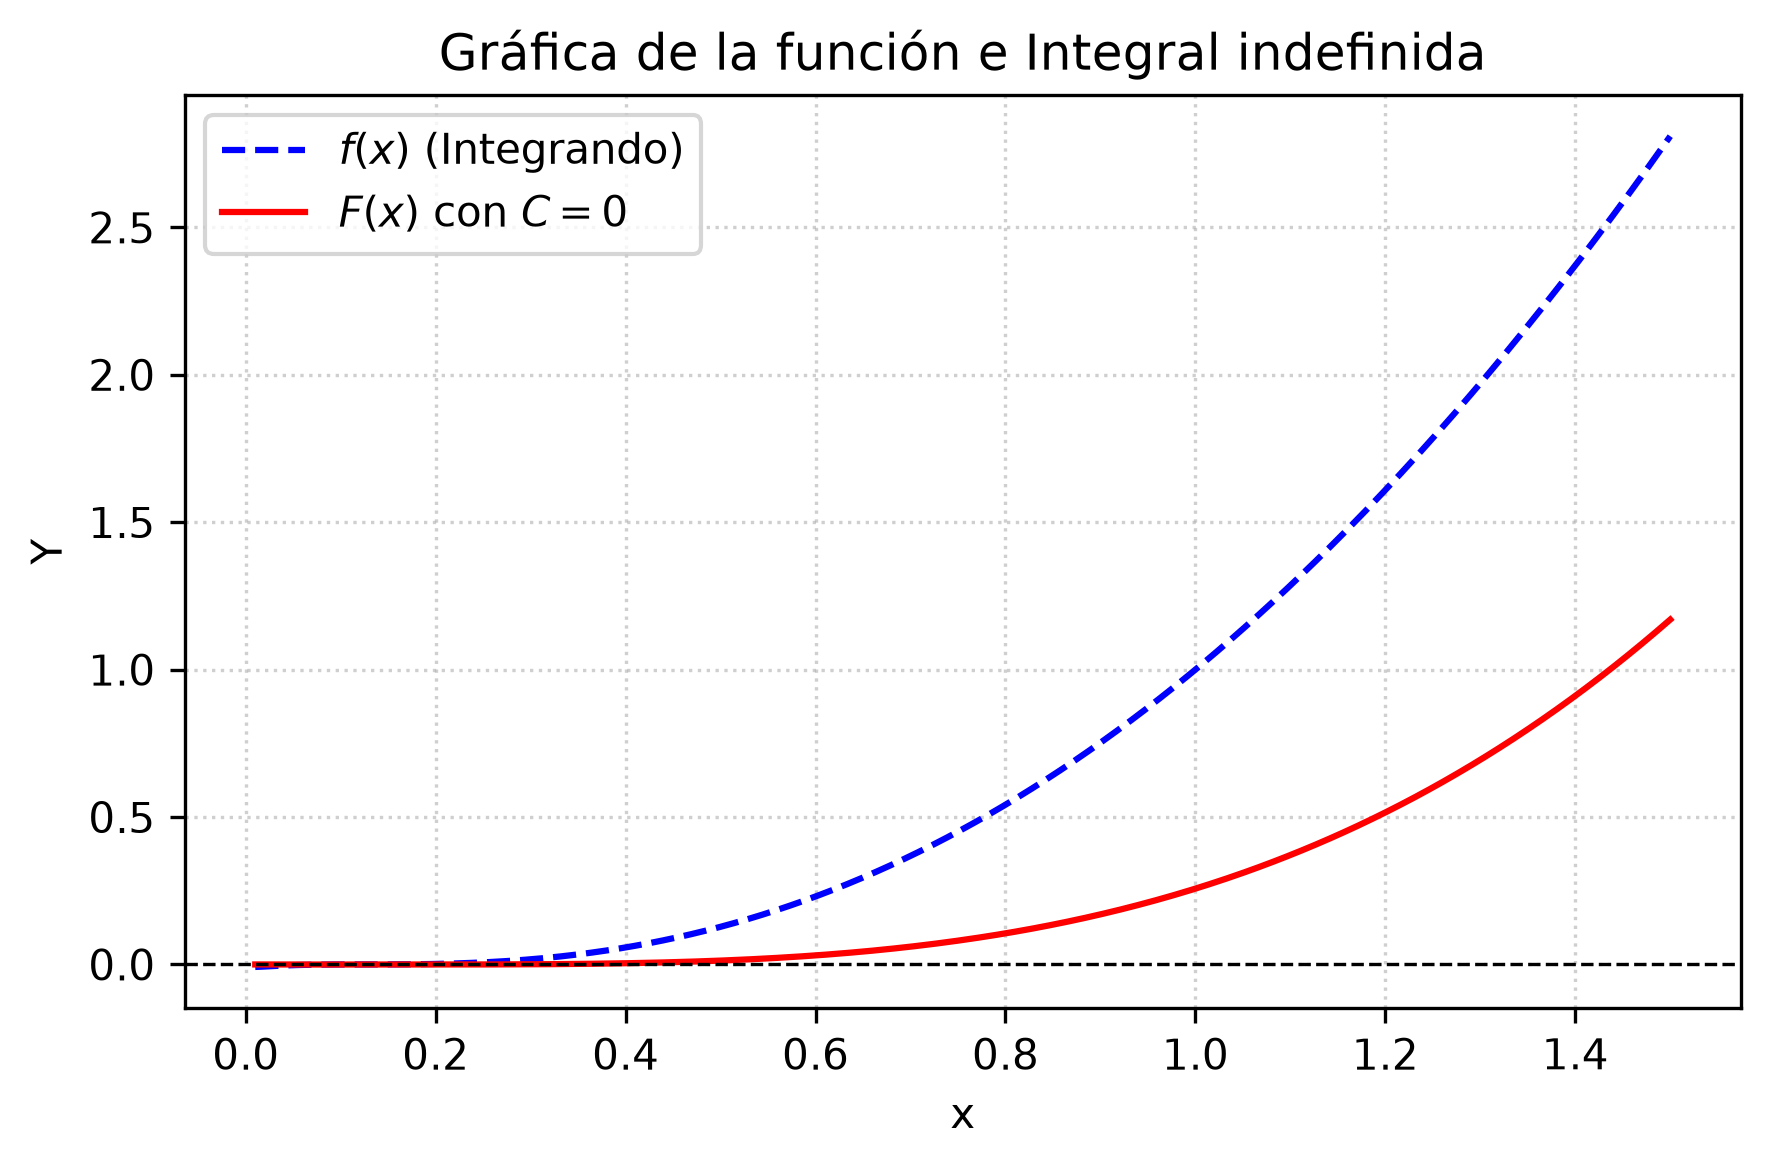
\includegraphics[width=\columnwidth]{semana_05/graficas/SEM05_P02_grafica.png}
	\caption{Representación gráfica de $f(x)$ y su antiderivada $F(x)$ evaluada para la constante de integración $C = 0$ (Problema 02).}
	\label{fig:problema02}
\end{figure}
